\documentclass[a4paper,12pt]{article} 
\usepackage{geometry}
\geometry{
	a4paper,
	total={170mm,257mm},
	left=20mm,
	top=20mm,
}
\usepackage{titlesec}
\titlelabel{\thetitle.\quad} %точка в section

%%% Работа с русским языком
\usepackage{cmap}                           % поиск в PDF
\usepackage{mathtext} 			 	       % русские буквы в формулах
\usepackage[T2A]{fontenc}               % кодировка
\usepackage[utf8]{inputenc}              % кодировка исходного текста
\usepackage[english,russian]{babel}  % локализация и переносы

%Математика
\usepackage{amsmath,amsfonts,amssymb,amsthm,mathtools} % AMS
\usepackage{icomma} % "Умная" запятая

%% Шрифты
\usepackage{euscript}	 % Шрифт Евклид
\usepackage{mathrsfs} % Красивый матшрифт

%% Команды
\DeclareMathOperator{\const}{\mathop{const}}

%% Перенос знаков в формулах
\newcommand*{\hm}[1]{#1\nobreak\discretionary{}
	{\hbox{$\mathsurround=0pt #1$}}{}}

%%% Заголовок
\author{Шерхалов Денис Б02-204}
\title{Лабораторная работа 2.1.1 \\
	\textbf{Измерение удельной теплоёмкости воздуха при постоянном давлении}}
\date{\today}

\begin{document}
	
	{\Large \maketitle}

	\paragraph*{Цель работы:} измерить повышение температуры воздуха в зависимости от мощности подводимого тепла и расхода при стационарном течении через трубу; исключив тепловые потери, по результатам измерений определить теплоёмкость воздуха при постоянном давлении.
	\paragraph*{В работе используются:} теплоизолированная стеклянная трубка; электронагреватель; источник питания постоянного тока; амперметр, вольтметр (цифровые мультиметры); термопара, подключенная к микровольтметру; компрессор; газовый счётчик;
	секундомер.
	
	\section{Введение}
	
	Теплоёмкость тела в некотором процессе определяется как их отношение: 
	\begin{equation*}
		C = \frac{\delta Q}{dT}
		\eqno(1)
	\end{equation*}
	
	Необходимо, чтобы количество тепла, затрачиваемое на нагревание исследуемого тела, существенно превосходило тепло, расходуемое на нагревание самого калориметра, а также на потери тепла из установки.
	
	Для увеличения количества нагреваемого газа при неизменных размерах установки в нашей работе исследуемый газ (воздух) продувается через калориметр, внутри которого установлен нагреватель. При этом
	измеряются мощность нагревателя, масса воздуха, протекающего в единицу
	времени (расход), и приращение его температуры.
	
	\begin{figure}[h!]
		\centering{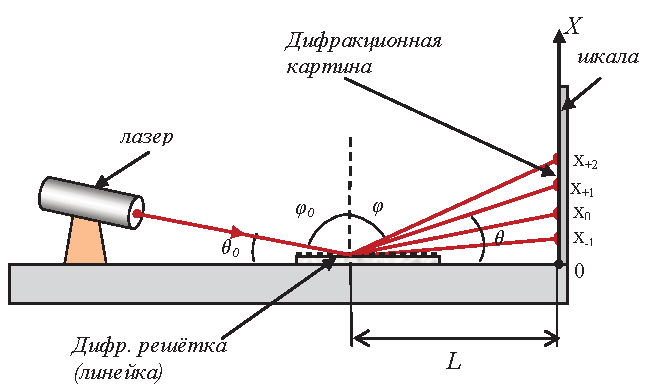
\includegraphics[width=0.5\textwidth]{pic2.jpg}}
		\caption[]{\label{fig:1} Нагрев газа при течении по трубе}
	\end{figure}

	Рассмотрим газ, протекающий стационарно слева направо через трубу постоянного сечения, в которой установлен нагревательный элемент (см. рис. 1). Пусть за некоторое время $dt$ через калориметр прошла малая порция газа массой $dm=q \, dt$, где $q$ [кг/с] — массовый расход газа в трубе. Если мощность нагрева равна $N$, мощность тепловых потерь на обмен с окружающей средой $N_{пот}$, то порция
	получила тепло $\delta Q = (N-N_{пот})dt$. С другой стороны, по определению теплоёмкости (1): $\delta Q = c \, dm \Delta T$, где $\Delta T = T_{2}-T_{1}$ — приращение температуры	газа, и $c$ — удельная (на единицу массы) теплоёмкость газа в рассматриваемом процессе. При малых расходах газа и достаточно большом диаметре
	трубы перепад давления на её концах мал, поэтому можно принять, что $P_{1} \approx P_{2} = P_{0}$, где $P_{0}$ — атмосферное давление. Следовательно, в условиях опыта
	измеряется удельная теплоёмкость при постоянном давлении $c_{P}$. Таким образом, получаем 
	\begin{equation*}
		c_{P} = \frac{N-N_{пот}}{q\Delta T}
		\eqno(2)
	\end{equation*}
	
	\subparagraph*{Экспериментальная установка:}
	
	Схема установки изображена на рис. 2. Воздух, нагнетаемый компрессором, прокачивается через калориметр. Калориметр представляет собой стеклянную цилиндрическую трубку с двойными стенками, запаянными с торцов.
	
	\begin{figure}[h!]
		\centering{\includegraphics[width=0.5\textwidth]{pic3.jpg}}
		\caption[]{\label{fig:2} Схема экспериментальной установки}
	\end{figure}

	
	Нагреватель в виде намотанной на пенопласт нихромовой проволоки расположен внутри калориметра непосредственно в воздушном потоке. Нагрев проволоки производится от регулируемого источника постоянного тока (ИП).
	Напряжение $U$ на нагревателе и ток $I$ через него регистрируются цифровыми мультиметрами. Таким образом, мощность нагрева равна
	\begin{equation*}
		N = UI
		\eqno(3)
	\end{equation*}

	Для измерения разности температур $\Delta T$ служит медно-константановая
	термопара. Один спай термопары расположен в струе воздуха, входящего в
	калориметр, и находится при комнатной температуре, а второй — в струе выходящего нагретого воздуха. Константановая проволока термопары расположена внутри калориметра, а медные проводники подключены к цифровому вольтметру. Возникающая в термопаре ЭДС $\varepsilon$ пропорциональна разности температур $\Delta T$ спаев: 
	\begin{equation*}
		\varepsilon =\beta \Delta T
		\eqno(4)
	\end{equation*}

	где $\beta = 40.7 \frac{мкВ}{К}$ — чувствительность медно-константановой термопары в рабочем диапазоне температур (20–30 $^\circ C$ ). ЭДС регистрируется с помощью микровольтметра.
	
	Объём воздуха, прошедшего через калориметр, измеряется газовым счётчиком ГС. Для регулировки расхода служит кран К. Время $\Delta t$ прохождения
	некоторого объема $\Delta V$ воздуха измеряется секундомером. Объёмный расход равен $\frac{\Delta V}{\Delta t} $, массовый расход может быть найден как 
	\begin{equation*}
		q = \rho_{0} \frac{\Delta V}{\Delta t}
		\eqno(5)
	\end{equation*}
	
	где $\rho_{0}$ — плотность воздуха при комнатной температуре, которая в свою очередь может быть получена из уравнения Менделеева–Клапейрона: $\rho_{0}= \frac{\mu P_{0} }{R T_{0}},$ где $P_{0}$ — атмосферное давление, $T_{0}$ — комнатная температура (в Кельвинах), $\mu = 29,0 {г/моль}$ — средняя молярная масса (сухого) воздуха.
	
	Учитывая особенности устройства калориметра, следует ожидать, что мощность нагревателя расходуется не только на нагрев массы прокачиваемого воздуха, но и частично теряется за счет нагрева внутренних стенок термостата и рассеяния тепла через торцы термостата. Можно предположить, что при небольшом нагреве ($\Delta T \ll T_{0}$) мощность потерь тепла $N_{пот}$ прямо пропорциональна разности температур:
	\begin{equation*}
		N_{пот} = \alpha \Delta T
		\eqno(6)
	\end{equation*}
	
	где $\alpha$ — некоторая константа. При этом условии основное соотношение (2) принимает вид 
	\begin{equation*}
		N = (C_{P}q +\alpha)\Delta T
		\eqno(7)
	\end{equation*}

	Следовательно, при фиксированном расходе воздуха ($q = \const$) подводимая мощность и разность температур связаны прямой пропорциональностью ($\Delta T(N)$ -- линейная функция).

	\section{Выполнение}
	
	\begin{enumerate}
		\item Подготовим к работе газовый счетчик: проверим, что он заполнен  водой, установим счётчик по уровню. Охладим калориметр до комнатной температуры. Включим вольтметр, предназначенный для измерения ЭДС термопары. 
		
		\item Запишем показания комнатной температуры и давления. $$T_{0} = 295.35 \; K, P_{0} = 98430 \pm 5 \; {Па} $$
		
		\item Установим максимальный расход воздуха на газовом счётчике -- $5$л за $30 \pm 0.5$с. Определим массовый расход воздуха $q_{0}$ [г/с].
		
		$$q_0 = \rho_0 \frac{\Delta V}{\Delta t} = \frac{\mu P_0}{RT_0} \frac{\Delta V}{\Delta t}$$
		
		Относительная погрешность косвенных измерений может быть найдена по формуле $$\sigma_{q_0} = \sqrt{\sigma_{T_0}^2 + \sigma_{P_0}^2 + \sigma_t^2}$$ 
		
		$$\frac{\Delta V_0}{\Delta t_0} = 0.1667\pm0.0027 \; \frac{л}{с} ,\quad  q_0 = 0.1939 \pm 0.0032 \; \frac{г}{с} $$
		
		\item Оценим величину тока нагревателя $I_{0}$, требуемого для нагрева воздуха на $\delta T = 1 {К}$.
		
		Определим теоретическое значение удельной теплоемкости воздуха при постоянном давлении $C_{m, P}^{теор} \; \frac{Дж}{г\cdot K}$, считая воздух идеальным двухатомным газом: $$C_{m, P}^{теор} = \frac{3.5R}{\mu} \approx 1003 \; \frac{Дж}{кг\cdot K}$$
		
		Оценим минимальную мощность $N_0$, необходимую для нагрева газа при максимальном расходе. $N_{0} = c_{p}q\Delta T + N_{пот} \approx c_{p}q\Delta T \approx 0.194$ Вт.
		
		Учитывая, что сопротивление проволоки нагревателя составляет приблизительно $R_{н} \approx 29$ Ом, искомое значение тока $I_{0} = \sqrt{\frac{N_{0}}{R_{н}}} \approx 0.08 \; {А}.$
		
		\item Отметим, что погрешности последующих измерений таковы:
		$$\Delta I = 0.05\; мA, \quad \Delta U = 0.5 \; мВ, \quad \Delta \varepsilon = 1 \; \mu В$$
		Следовательно, оценим погрешности косвенных величин так: 
		$$\Delta N = U \Delta I + I \Delta U, \quad \delta T = \dfrac{\Delta \varepsilon}{\beta} = 0.02 K$$
		
		\item Проведем измерение зависимости разности температур от мощности нагрева $\Delta T(N)$ при максимальном расходе воздуха $q_0 = 0.1939 \pm 0.0032 \frac{г}{с}$. (Таблица №1, график №1).
		
		\begin{table}[h!] 
			\caption{Измерение $\Delta T (N) \; {при} \; q_0 = 0.1939 \pm 0.0032 \frac{г}{с}$}
			\begin{center}
				\begin{tabular}{|*{6}{l|}}
					\hline
					$U$, В & $I$, мА & $N$, мВт & $\Delta N$, мВт & $\varepsilon$, мВ & $\Delta T$, K\\ \hline
					3.458 & 121.9 & 421.5 & 0.2 & 0.071 & 1.47 \\ \hline
					4.526 & 159.4 & 721.4 & 0.3 & 0.120 & 2.95 \\ \hline
					5.880 & 206.9 & 1216.6 & 0.4 & 0.205 & 5.04 \\ \hline
					7.820 & 274.8 & 2148.9 & 0.5 & 0.359 & 8.82 \\ \hline
				\end{tabular}
			\end{center}
		\end{table}
	
		\begin{figure}[h!]
			\centering{\includegraphics[width=1\textwidth]{gr1.png}}
			\caption[]{\label{fig:3} График №1}
		\end{figure}
	
		Коэффициент наклона графика №1: $k_1 = 4.104\pm0.002 \frac{K}{Вт}$
			
		\item Завершив первую серию измерении, охладим калориметр до комнатной температуры.
		Для этого отключим источник питания нагревателя, откроем кран К и продуем калориметр при максимальном расходе воздуха до тех пор, пока показания ЭДС не достигнут нуля.
		
		Повторим измерения при другом расходе. Установим расход воздуха на газовом счётчике -- $5$л за $61 \pm 0.5$с. Определим массовый расход воздуха $q_1$ [г/с].
		
		$$\frac{\Delta V_1}{\Delta t_1} = 0.0820 \pm 0.0007 \; \frac{л}{с} ,\quad  q_1 = 0.0955 \pm 0.0008 \; \frac{г}{с} $$
		
		\item Проведем измерение зависимости разности температур от мощности нагрева $\Delta T(N)$ при максимальном расходе воздуха $q_1 = 0.0955 \pm 0.0008 \; \frac{г}{с}$. (Таблица №2, график №2).
		
		\begin{table}[h!] 
			\caption{Измерение $\Delta T (N) \; {при} \; q_1 = 0.0955 \pm 0.0008 \; \frac{г}{с}$}
			\begin{center}
				\begin{tabular}{|*{6}{l|}}
					\hline
					$U$, В & $I$, мА & $N$, мВт & $\Delta N$, мВт &$\varepsilon$, мВ & $\Delta T$, K\\ \hline
					3.499 & 123.3 & 431.4 & 0.2 & 0.129 & 3.17 \\ \hline
					4.417 & 155.5 & 686.8 & 0.3 & 0.205 & 5.04 \\ \hline
					5.511 & 193.8 & 1068.0 & 0.4 & 0.313 & 7.69 \\ \hline
					6.138 & 215.8 & 1304.6 & 0.4 & 0.388 & 9.53 \\ \hline
				\end{tabular}
			\end{center}
		\end{table}

		\begin{figure}[h!]
			\centering{\includegraphics[width=1\textwidth]{gr2.png}}
			\caption[]{\label{fig:4} График №2}
		\end{figure}
	
		Коэффициент наклона графика №2: $k_2 = 7.099\pm0.002 \frac{K}{Вт}$
		
		\item Остаётся найти $С_p$, пользуясь формулой (7).
		\\ $k_1 = 4.104\pm0.002 \frac{K}{Вт} \; \Rightarrow \; \left(\dfrac{N}{\Delta T}\right)_1 = \dfrac{1}{k_1} = 0.2437 \pm 0.0001 \frac{Вт}{К}$
		\\ $k_2 = 7.099\pm0.002 \frac{K}{Вт} \; \Rightarrow \; \left(\dfrac{N}{\Delta T}\right)_2 = \dfrac{1}{k_2} = 0.14086 \pm 0.00004 \frac{Вт}{К}$

		Построим график зависимости $\dfrac{N}{\Delta T},\;\; \frac{мВт}{К}$  от  $q,\;\; \frac{г}{c}$ (Таблица №3, график №3)
		
		\begin{table}[h!] 
			\caption{$\frac{N}{\Delta T} \frac{мВт}{К} \;\;{от}\;\; q \; \frac{г}{с}$}
			\begin{center}
				\begin{tabular}{|*{4}{l|}}
					\hline
					$\dfrac{N}{\Delta T}$, $\frac{мВт}{К}$ & $\Delta \left(\dfrac{N}{\Delta T}\right)$, $\frac{мВт}{К}$ & $q$, $\frac{г}{с}$ & $\Delta q$, $\frac{г}{с}$ \\ \hline
					243.7 & 0.1 & 0.1939 & 0.0032 \\ \hline
					140.86 & 0.04 & 0.0955 & 0.0008 \\ \hline
				\end{tabular}
			\end{center}
		\end{table}
		\begin{figure}[h!]
			\centering{\includegraphics[width=1\textwidth]{gr3.png}}				\caption[]{\label{fig:5} График №3}
		\end{figure}

		Коэффициент наклона графика №3: $c_p = k_3 = 1045 \pm 40 \frac{Дж}{кг\cdot К}$.
	\end{enumerate}

	\section{Вывод}
	
	В ходе эксперимента при использовании знаний полученных в ходе курса термодинамики было получено значение удельной массовой теплоёмкости воздуха при постоянном давлении. Полученное значение $С_{m, P} = 1045 \pm 40 \frac{Дж}{кг\cdot К}$ хорошо совпало с теоретическим $C_{m, P}^{теор} = 1003 \; \frac{Дж}{кг\cdot K}$. В свою очередь, табличное значение для удельной теплоёмкости воздуха варьируется: $C_{m, P}^{табл} = 1007-1030 \; \frac{Дж}{кг\cdot K}$ при комнатной температуре в зависимости от влажности (нулевая -- $100\%$).
	\\ Неполное совпадение результата вызвано, вероятно, во-первых, тем, что воздух -- это не совсем смесь идеальных двухамтомных газов, как минимум в силу наличия в воздухе водяного пара, а во-вторых тем, что установление идеального равновесия требует слишком большого времени ожидания, в связи с чем снимаемые значения $I$, $U$, $\varepsilon$ -- не совсем равновесные.
	
\end{document}